\documentclass[12pt, twocolumn]{article}
\usepackage{threeDipole}

\title{Three Magnetic Dipole Problem}
\author{Callebe R. Reis}
\date{\today}

\begin{document}
\maketitle

\tableofcontents

\section{Introduction}
Magnetic systems often exhibit nonlinear responses to external magnetic fields. This means, for example that the relation between an applied magnetic field and the resulting magnetization of a magnetizable material is not linearly proportional, which can induce a variety of interesting phenomena. Many examples can be mentioned, for example the as chaotic behavior of the system, autoresonance, and turbulence, such as in earth\textquotesingle s magneto tail~\cite{nonlinearResponse,Bratman1983,Loeb1986,VerandaM,Brunton2017,Chang1999}. 

%Nonlinearity can arise due to various factors such as magnetic anisotropy, domain wall motion, and magnetic interactions~\cite{HORVATH2022119279}.

Previous works shown that the influence of small fluctuations in a system composed of two magnetic dipoles can lead to two different behaviors: the dipoles fluctuate around stable fixed points (with low amplitude fluctuations), or stochastic reversals occurs between stable fixed points (with strong fluctuations). Low energy fluctuations lead to disjoint basins of attraction near stable fixed points, while higher fluctuations connect basins (including an unstable fixed point) with stochastic reversals and Poisson-distributed waiting time~\cite{santos2019dinamica, StochasticReversalDynamics}. 
%In this work, we are interested in the second case, by each the system presents a rather unexpected behavior. 

One may suggest that, for a system composed of two magnetic dipoles, there exists a nonlinear coupling, and the problem presents two different time scales depending on the magnitudes of the magnetic interactions, because they are of different nature~\cite{LAROZE20081440}.
% As we\textquotesingle ll see, such a phenomenon occurs for the single magnetic dipole in an oscillating magnetic field. 

This work focuses on investigating the dynamics of a system composed of three equidistantly spaced bar magnets fixed on a table, each free to rotate about its center. 

In order to better analyze this system, we consider the length of the magnets to be small compared to the distance between them, allowing us to approximate the bar magnets for magnetic dipoles.

We studied the case where two magnets are much stronger than the third one, and, taking sufficient approximations, we were able to investigate the system as a single magnet in a homogeneous magnetic field whose direction oscillates in time.

This simplified system can exhibit unexpected and chaotic behavior when, from an equilibrium initial state, a small perturbation that can increase kinetic energy of the system is applied to the small magnet through the oscillations of the external magnetic field. This interesting behavior occurs at specific values of the physical parameters, such as the system\textquotesingle s natural frequency and the frequency at which the magnetic field oscillates.

Comprehending the mechanisms by which kinetic energy transfers among the magnetic field and the magnet was the original motivation to this project. Having a good understanding of this phenomenon is crucial for gaining insights into the dynamics of magnetic systems and their potential applications.

% was extensivelly studied in~\cite{yung1970analytic, ku2016interaction, santos2019dinamica}, in~\cite{yung1970analytic} equations for the motion of two dipoles are derived, and~\cite{ku2016interaction, santos2019dinamica} investigated the damping version as well as the system in a presence of a external magnetic field.



% As any dynamical system, there could be stable or unstable points of equilibrium for this system, and as shown in the work of Carlos for the system with two magnetic dipoles there are eigth equilibrium points, and for a ring made out of magnetic dipoles.

\subsection{Theoretical model}

A single magnetic dipole with magnetic moment $\boldsymbol{m}$, generates a magnetic field at a distance $\boldsymbol{r}$, accordingly to the expression: 
\begin{equation}
    \boldsymbol{B} = \dfrac{3\mu_0}{4 \pi r^3}\bigg[ (\boldsymbol{m \cdot \hat{r}})\boldsymbol{\hat{r}} - \dfrac{1}{3}\boldsymbol{m} \bigg],
    \label{eq:MagneticFieldDipole}
\end{equation}
where, $\mu_0$ is the magnetic permeability of the medium. 

If subjected to an external magnetic field $\boldsymbol{B}_{ext}$, the magnetic dipole experiences a torque: 
\begin{equation}
    \boldsymbol{\tau} = \boldsymbol{m} \times \boldsymbol{B}_{ext}.
    \label{eq:NewtonSecondLaw}
\end{equation}

Let us consider a system composed of three magnetic dipoles, each placed at a vertex of an equilateral triangle and equally spaced. The magnetic field generated by each of the dipoles is felt by the other two. By adding the torques at the dipole $i$, generated by the dipoles $j$ and $k$, we find that, the resulting torque on dipole $i$ is:
\begin{equation}
    \begin{aligned}
        \boldsymbol{\tau}_i &= \boldsymbol{\tau}_{ij} + \boldsymbol{\tau}_{ik}\\
            & =  \boldsymbol{m}_i \times \boldsymbol{B}_{j i}+\boldsymbol{m_i} \times \boldsymbol{B}_{k i}\\
            &= \boldsymbol{m}_i \times \boldsymbol{B}_{res}
    \end{aligned}
    \label{eq:Torques}
\end{equation}
where, $\boldsymbol{B}_{res}$, represents the resulting magnetic field generated by the two dipoles $j$ and $k$. 

In this work we analyze a model where two dipoles have much greater moments of inertia than the third, and that the resulting magnetic field generated by the two heavy dipoles is approximately homogeneous, i.e,

\begin{equation}
    \begin{aligned}
        % I_1 & \ll I_2,\\
        % I_1 & \ll I_3,\\
        \boldsymbol{B}_{res} &= B(\cos(\theta_1),\sin(\theta_1), 0),
    \end{aligned}
    \label{eq:Hipotesys}
\end{equation}
where $\theta_1$ represents the angular displacement of the magnetic field.

If the smaller dipole has magnetic moment given by:
\begin{equation}
    \boldsymbol{m}_1 = m_1 (\cos(\theta), \sin(\theta), 0),
    \label{eq:MagneticMoment}
\end{equation}
then, because $\boldsymbol{B}_{res}$ and $\boldsymbol{m_1}$ are in the same plane, the torque at the smaller dipole will have only components in the direction of $\boldsymbol{\hat{z}}$.

Therefore, in the above conditions, and accordingly to Newton~\textquotesingle s Second Law of motion for spinning objects, the equation~(\ref{eq:Torques}) gives rise to the equation of motion of a single dipole:
\begin{equation}
    \begin{aligned}
        &\tau_1 - I_1 \ddot{\theta} = 0\\
        &I \ddot{\theta} + m_1 B \sin(\theta - \theta_1) = 0        
    \end{aligned}
\end{equation}
and calling
\begin{equation}
    \eta^2 = m_1 B/I 
\end{equation} 
then
\begin{equation}
    \ddot{\theta} +\eta^2 \sin(\theta - \theta_1) = 0.
    \label{eq:EquationOfMotion}
\end{equation}
We remark that, the equation (\ref{eq:EquationOfMotion}) is very similar to the pendulum equation, except for the $\theta_1$ parameter.

% \subsection{Forced System}

In general, the two heavy dipoles do not remain static, but oscillate with small amplitude:
\begin{equation}
    \theta_1(t) = \varepsilon \sin(\Omega t)
\end{equation}
Therefore, generating an oscillating magnetic field, with frequency $\Omega$, which turns equation (\ref{eq:EquationOfMotion}) into the equation (\ref{eq:MotionWithOmega}).
\begin{equation}
    \ddot{\theta} +\eta^2 \sin(\theta - \varepsilon \sin(\Omega t)) = 0.
    \label{eq:MotionWithOmega}
\end{equation}
% Making the following change of variables:
% \begin{equation}
%     \begin{aligned}
%         \phi &= \theta - \varepsilon \sin(\Omega t),\\
%         \ddot{\phi} &= \ddot{\theta} + \varepsilon \Omega^2 \sin(\Omega t)
%     \end{aligned}
% \end{equation}
% resulting in, 
% \begin{equation}
%     \ddot{\phi} + \eta^2 \sin(\phi) =\Omega^2 \varepsilon \sin(\Omega t)
% \end{equation}
% which is the equation of a forced pendulum.

% (to be continued)

\section{Numerical Methods}
\subsection{Runge-Kutta 4th order}~\label{sec:RK4}

In order to investigate equation (\ref{eq:EquationOfMotion}) numerically, we used the iterative method of Runge-Kutta of fourth order (RK4), which has a low computational cost, and fourth order accuracy, i.e, at each iteration the error is at most $\mathcal{O}(h^4)$, where $h$ is the integration step.

Before applying the method, we have transformed the second order differential equation of motion of dipole (\ref{eq:EquationOfMotion}), into two first order differential equation by making the transformations:

\begin{equation}
    \begin{aligned}
        x_1 &= \theta,\\
        x_2 &= \dot{\theta}, 
    \end{aligned}
\end{equation}
leading to the system of first order differential equations below:
\begin{equation}
    \begin{cases}
        \dot{x_1} &= x_2,\\
        \dot{x_2} &= -\eta^2 \sin(x_1 - \varepsilon \sin(\Omega t)),
    \end{cases}
\end{equation}
We used $h=10^{-4}$ for most simulations, equation (\ref{eq:EquationOfMotion}) and $h = 0.05$ for the construction of the bifurcation diagrams.

\subsection{Simpson\textquotesingle s 1/3 rule and Fourier transform}
After solving the differential equation numerically using the \hyperref[sec:RK4]{RK4} method, we used the Simpson\textquotesingle s $1/3$ rule, equation (\ref{eq:SimpsonsRule}), to numerically integrate the Fourier transform, equation~\ref{eq:FourierTransform}.
\begin{equation}
    \mathcal{F}\{f(t)\}= \dfrac{2}{T}\int_{0}^{T} f(t) e^{- i \xi t}dt
    \label{eq:FourierTransform}
\end{equation}
% \begin{equation}
    \begin{multline}
        \int_{a}^{b} f(x) dx = \dfrac{1}{3} h\bigg[ f(a) + 
         4\sum^{n/2}_{n=1}f(x_{2i-1}) \\
         + 2 \sum^{n/2 - 1}_{n=1}f(x_{2i})+f(b) \bigg]        
    \label{eq:SimpsonsRule}
\end{multline}
\subsection{Bifurcation diagrams}

For creating the bifurcation diagrams, figures~\ref{fig:bif005} and~\ref{fig:bif05}, we vary the frequency of the magnetic field, $\Omega$, from $-3$ to $3$ using a step of $0.01$, and for each frequency $\Omega$ we solved equation (\ref{eq:EquationOfMotion}) for $t \in [0,500]$ using the \hyperref[sec:RK4]{RK4} method, then applied the Fourier transform and filtered out the frequencies with amplitude less than $20\%$ of the maximum amplitude. Finally, for each $\Omega$ we plotted the frequencies obtained from the Fourier transform, $\omega$, creating a graph, $(\Omega,\omega)$ where the $\omega$ frequencies represent the frequency response of the system.  


\section{First Results}

In this Section, we\textquotesingle ll briefly discuss the dynamics of the equation (\ref{eq:EquationOfMotion}), with mostly numerical results. 

The dipole\textquotesingle s dynamics was studied for small amplitude of oscillation of the magnetic field. We used two main values for the parameter $\varepsilon$, $\varepsilon = 0.05$ and $\varepsilon = 0.5$, and the following initial conditions for both cases:
\begin{equation}
    \begin{cases}
        \theta (0) &= 1\\        
        \dot{\theta}(0) &= 0
    \end{cases}
\end{equation} 
In the former case, $\varepsilon = 0.05$, we verify that the dipole\textquotesingle s movement was periodic for all the values of the frequency of the magnetic field $\Omega$ in $[-3,3]$, and as expected, the dipole behaved like a simple pendulum. 

However, for the latter case, $\varepsilon = 0.5$, the dipole\textquotesingle s movement was much more complex, and for some subintervals in the frequency range in $[-3,3]$, the movement was not periodic, figure \ref{fig:omega075}, and maybe not even limited. 

In the cases where the movement was oscillatory, the oscillation frequency was not comparable to the frequency of the magnetic field, and for the most time, the frequency of the movement was the natural frequency of the system. 

\begin{figure}[ht]
    \scalebox{0.7}{% GNUPLOT: LaTeX picture with Postscript
\begingroup
  \makeatletter
  \providecommand\color[2][]{%
    \GenericError{(gnuplot) \space\space\space\@spaces}{%
      Package color not loaded in conjunction with
      terminal option `colourtext'%
    }{See the gnuplot documentation for explanation.%
    }{Either use 'blacktext' in gnuplot or load the package
      color.sty in LaTeX.}%
    \renewcommand\color[2][]{}%
  }%
  \providecommand\includegraphics[2][]{%
    \GenericError{(gnuplot) \space\space\space\@spaces}{%
      Package graphicx or graphics not loaded%
    }{See the gnuplot documentation for explanation.%
    }{The gnuplot epslatex terminal needs graphicx.sty or graphics.sty.}%
    \renewcommand\includegraphics[2][]{}%
  }%
  \providecommand\rotatebox[2]{#2}%
  \@ifundefined{ifGPcolor}{%
    \newif\ifGPcolor
    \GPcolortrue
  }{}%
  \@ifundefined{ifGPblacktext}{%
    \newif\ifGPblacktext
    \GPblacktexttrue
  }{}%
  % define a \g@addto@macro without @ in the name:
  \let\gplgaddtomacro\g@addto@macro
  % define empty templates for all commands taking text:
  \gdef\gplbacktext{}%
  \gdef\gplfronttext{}%
  \makeatother
  \ifGPblacktext
    % no textcolor at all
    \def\colorrgb#1{}%
    \def\colorgray#1{}%
  \else
    % gray or color?
    \ifGPcolor
      \def\colorrgb#1{\color[rgb]{#1}}%
      \def\colorgray#1{\color[gray]{#1}}%
      \expandafter\def\csname LTw\endcsname{\color{white}}%
      \expandafter\def\csname LTb\endcsname{\color{black}}%
      \expandafter\def\csname LTa\endcsname{\color{black}}%
      \expandafter\def\csname LT0\endcsname{\color[rgb]{1,0,0}}%
      \expandafter\def\csname LT1\endcsname{\color[rgb]{0,1,0}}%
      \expandafter\def\csname LT2\endcsname{\color[rgb]{0,0,1}}%
      \expandafter\def\csname LT3\endcsname{\color[rgb]{1,0,1}}%
      \expandafter\def\csname LT4\endcsname{\color[rgb]{0,1,1}}%
      \expandafter\def\csname LT5\endcsname{\color[rgb]{1,1,0}}%
      \expandafter\def\csname LT6\endcsname{\color[rgb]{0,0,0}}%
      \expandafter\def\csname LT7\endcsname{\color[rgb]{1,0.3,0}}%
      \expandafter\def\csname LT8\endcsname{\color[rgb]{0.5,0.5,0.5}}%
    \else
      % gray
      \def\colorrgb#1{\color{black}}%
      \def\colorgray#1{\color[gray]{#1}}%
      \expandafter\def\csname LTw\endcsname{\color{white}}%
      \expandafter\def\csname LTb\endcsname{\color{black}}%
      \expandafter\def\csname LTa\endcsname{\color{black}}%
      \expandafter\def\csname LT0\endcsname{\color{black}}%
      \expandafter\def\csname LT1\endcsname{\color{black}}%
      \expandafter\def\csname LT2\endcsname{\color{black}}%
      \expandafter\def\csname LT3\endcsname{\color{black}}%
      \expandafter\def\csname LT4\endcsname{\color{black}}%
      \expandafter\def\csname LT5\endcsname{\color{black}}%
      \expandafter\def\csname LT6\endcsname{\color{black}}%
      \expandafter\def\csname LT7\endcsname{\color{black}}%
      \expandafter\def\csname LT8\endcsname{\color{black}}%
    \fi
  \fi
    \setlength{\unitlength}{0.0500bp}%
    \ifx\gptboxheight\undefined%
      \newlength{\gptboxheight}%
      \newlength{\gptboxwidth}%
      \newsavebox{\gptboxtext}%
    \fi%
    \setlength{\fboxrule}{0.5pt}%
    \setlength{\fboxsep}{1pt}%
    \definecolor{tbcol}{rgb}{1,1,1}%
\begin{picture}(6480.00,4320.00)%
    \gplgaddtomacro\gplbacktext{%
      \csname LTb\endcsname%%
      \put(726,440){\makebox(0,0)[r]{\strut{}$-1$}}%
      \put(726,806){\makebox(0,0)[r]{\strut{}$-0.8$}}%
      \put(726,1172){\makebox(0,0)[r]{\strut{}$-0.6$}}%
      \put(726,1538){\makebox(0,0)[r]{\strut{}$-0.4$}}%
      \put(726,1904){\makebox(0,0)[r]{\strut{}$-0.2$}}%
      \put(726,2270){\makebox(0,0)[r]{\strut{}$0$}}%
      \put(726,2635){\makebox(0,0)[r]{\strut{}$0.2$}}%
      \put(726,3001){\makebox(0,0)[r]{\strut{}$0.4$}}%
      \put(726,3367){\makebox(0,0)[r]{\strut{}$0.6$}}%
      \put(726,3733){\makebox(0,0)[r]{\strut{}$0.8$}}%
      \put(726,4099){\makebox(0,0)[r]{\strut{}$1$}}%
      \put(858,220){\makebox(0,0){\strut{}$-3$}}%
      \put(1729,220){\makebox(0,0){\strut{}$-2$}}%
      \put(2600,220){\makebox(0,0){\strut{}$-1$}}%
      \put(3471,220){\makebox(0,0){\strut{}$0$}}%
      \put(4341,220){\makebox(0,0){\strut{}$1$}}%
      \put(5212,220){\makebox(0,0){\strut{}$2$}}%
      \put(6083,220){\makebox(0,0){\strut{}$3$}}%
    }%
    \gplgaddtomacro\gplfronttext{%
    \csname LTb\endcsname%%
    \put(152,2270){\rotatebox{-270}{\makebox(0,0){\strut{}$\omega $}}}%
    \put(3471,-112){\makebox(0,0){\strut{}$\Omega$}}%
  }%
    \gplbacktext
    \put(0,0){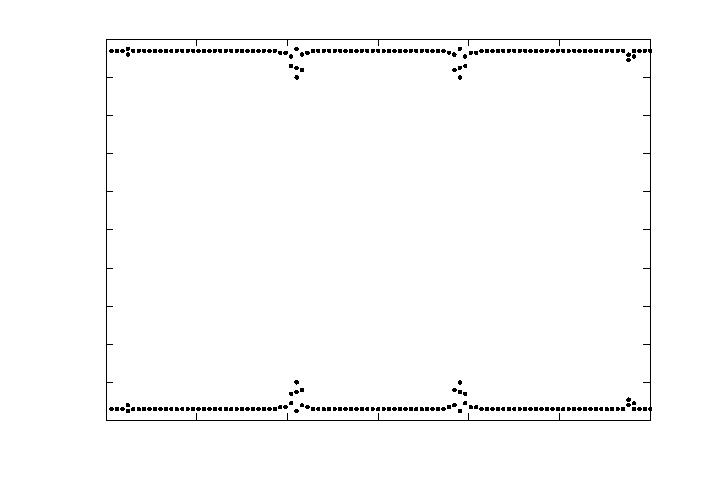
\includegraphics[width={324.00bp},height={216.00bp}]{images/FrequencyBifurcation005}}%
    \gplfronttext
  \end{picture}%
\endgroup
}
    \caption{Bifurcation diagram of frequencies from the oscillating magnetic field $\Omega$ and the response frequencies on the dipole $\omega$, for the case with $\varepsilon = 0.05$.}
    \label{fig:big005}
\end{figure}

\begin{figure}[ht]
    \scalebox{0.7}{% GNUPLOT: LaTeX picture with Postscript
\begingroup
  \makeatletter
  \providecommand\color[2][]{%
    \GenericError{(gnuplot) \space\space\space\@spaces}{%
      Package color not loaded in conjunction with
      terminal option `colourtext'%
    }{See the gnuplot documentation for explanation.%
    }{Either use 'blacktext' in gnuplot or load the package
      color.sty in LaTeX.}%
    \renewcommand\color[2][]{}%
  }%
  \providecommand\includegraphics[2][]{%
    \GenericError{(gnuplot) \space\space\space\@spaces}{%
      Package graphicx or graphics not loaded%
    }{See the gnuplot documentation for explanation.%
    }{The gnuplot epslatex terminal needs graphicx.sty or graphics.sty.}%
    \renewcommand\includegraphics[2][]{}%
  }%
  \providecommand\rotatebox[2]{#2}%
  \@ifundefined{ifGPcolor}{%
    \newif\ifGPcolor
    \GPcolortrue
  }{}%
  \@ifundefined{ifGPblacktext}{%
    \newif\ifGPblacktext
    \GPblacktexttrue
  }{}%
  % define a \g@addto@macro without @ in the name:
  \let\gplgaddtomacro\g@addto@macro
  % define empty templates for all commands taking text:
  \gdef\gplbacktext{}%
  \gdef\gplfronttext{}%
  \makeatother
  \ifGPblacktext
    % no textcolor at all
    \def\colorrgb#1{}%
    \def\colorgray#1{}%
  \else
    % gray or color?
    \ifGPcolor
      \def\colorrgb#1{\color[rgb]{#1}}%
      \def\colorgray#1{\color[gray]{#1}}%
      \expandafter\def\csname LTw\endcsname{\color{white}}%
      \expandafter\def\csname LTb\endcsname{\color{black}}%
      \expandafter\def\csname LTa\endcsname{\color{black}}%
      \expandafter\def\csname LT0\endcsname{\color[rgb]{1,0,0}}%
      \expandafter\def\csname LT1\endcsname{\color[rgb]{0,1,0}}%
      \expandafter\def\csname LT2\endcsname{\color[rgb]{0,0,1}}%
      \expandafter\def\csname LT3\endcsname{\color[rgb]{1,0,1}}%
      \expandafter\def\csname LT4\endcsname{\color[rgb]{0,1,1}}%
      \expandafter\def\csname LT5\endcsname{\color[rgb]{1,1,0}}%
      \expandafter\def\csname LT6\endcsname{\color[rgb]{0,0,0}}%
      \expandafter\def\csname LT7\endcsname{\color[rgb]{1,0.3,0}}%
      \expandafter\def\csname LT8\endcsname{\color[rgb]{0.5,0.5,0.5}}%
    \else
      % gray
      \def\colorrgb#1{\color{black}}%
      \def\colorgray#1{\color[gray]{#1}}%
      \expandafter\def\csname LTw\endcsname{\color{white}}%
      \expandafter\def\csname LTb\endcsname{\color{black}}%
      \expandafter\def\csname LTa\endcsname{\color{black}}%
      \expandafter\def\csname LT0\endcsname{\color{black}}%
      \expandafter\def\csname LT1\endcsname{\color{black}}%
      \expandafter\def\csname LT2\endcsname{\color{black}}%
      \expandafter\def\csname LT3\endcsname{\color{black}}%
      \expandafter\def\csname LT4\endcsname{\color{black}}%
      \expandafter\def\csname LT5\endcsname{\color{black}}%
      \expandafter\def\csname LT6\endcsname{\color{black}}%
      \expandafter\def\csname LT7\endcsname{\color{black}}%
      \expandafter\def\csname LT8\endcsname{\color{black}}%
    \fi
  \fi
    \setlength{\unitlength}{0.0500bp}%
    \ifx\gptboxheight\undefined%
      \newlength{\gptboxheight}%
      \newlength{\gptboxwidth}%
      \newsavebox{\gptboxtext}%
    \fi%
    \setlength{\fboxrule}{0.5pt}%
    \setlength{\fboxsep}{1pt}%
    \definecolor{tbcol}{rgb}{1,1,1}%
\begin{picture}(6480.00,4320.00)%
    \gplgaddtomacro\gplbacktext{%
      \csname LTb\endcsname%%
      \put(726,440){\makebox(0,0)[r]{\strut{}$-1$}}%
      \put(726,806){\makebox(0,0)[r]{\strut{}$-0.8$}}%
      \put(726,1172){\makebox(0,0)[r]{\strut{}$-0.6$}}%
      \put(726,1538){\makebox(0,0)[r]{\strut{}$-0.4$}}%
      \put(726,1904){\makebox(0,0)[r]{\strut{}$-0.2$}}%
      \put(726,2270){\makebox(0,0)[r]{\strut{}$0$}}%
      \put(726,2635){\makebox(0,0)[r]{\strut{}$0.2$}}%
      \put(726,3001){\makebox(0,0)[r]{\strut{}$0.4$}}%
      \put(726,3367){\makebox(0,0)[r]{\strut{}$0.6$}}%
      \put(726,3733){\makebox(0,0)[r]{\strut{}$0.8$}}%
      \put(726,4099){\makebox(0,0)[r]{\strut{}$1$}}%
      \put(858,220){\makebox(0,0){\strut{}$-3$}}%
      \put(1729,220){\makebox(0,0){\strut{}$-2$}}%
      \put(2600,220){\makebox(0,0){\strut{}$-1$}}%
      \put(3471,220){\makebox(0,0){\strut{}$0$}}%
      \put(4341,220){\makebox(0,0){\strut{}$1$}}%
      \put(5212,220){\makebox(0,0){\strut{}$2$}}%
      \put(6083,220){\makebox(0,0){\strut{}$3$}}%
    }%
    \gplgaddtomacro\gplfronttext{%
    \csname LTb\endcsname%%
    \put(152,2270){\rotatebox{-270}{\makebox(0,0){\strut{}$\omega $}}}%
    \put(3471,-112){\makebox(0,0){\strut{}$\Omega$}}%
  }%
 
    \gplbacktext
    \put(0,0){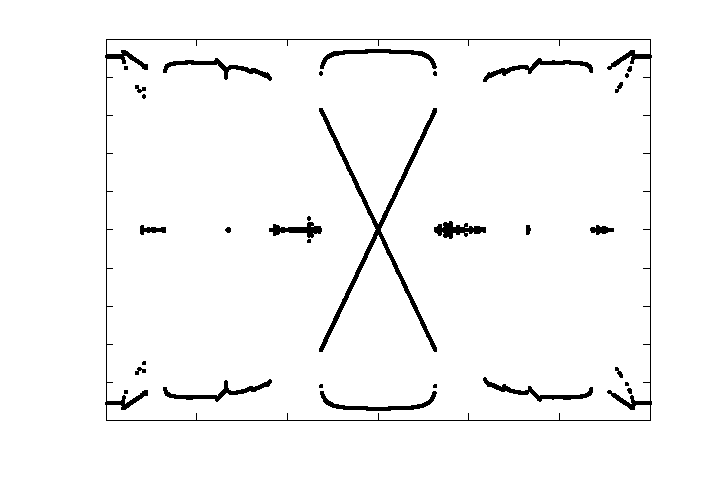
\includegraphics[width={324.00bp},height={216.00bp}]{images/FrequencyBifurcation}}%
    \gplfronttext
  \end{picture}%
\endgroup
}
    \caption{Bifurcation diagram of frequencies from the oscillating magnetic field $\Omega$ and the response frequencies on the dipole $\omega$, for the case with $\varepsilon = 0.5$.}
    \label{fig:bif05}
\end{figure}

\begin{figure*}
    \begin{subfigure}{\textwidth}
        % GNUPLOT: LaTeX picture with Postscript
\begingroup
  \makeatletter
  \providecommand\color[2][]{%
    \GenericError{(gnuplot) \space\space\space\@spaces}{%
      Package color not loaded in conjunction with
      terminal option `colourtext'%
    }{See the gnuplot documentation for explanation.%
    }{Either use 'blacktext' in gnuplot or load the package
      color.sty in LaTeX.}%
    \renewcommand\color[2][]{}%
  }%
  \providecommand\includegraphics[2][]{%
    \GenericError{(gnuplot) \space\space\space\@spaces}{%
      Package graphicx or graphics not loaded%
    }{See the gnuplot documentation for explanation.%
    }{The gnuplot epslatex terminal needs graphicx.sty or graphics.sty.}%
    \renewcommand\includegraphics[2][]{}%
  }%
  \providecommand\rotatebox[2]{#2}%
  \@ifundefined{ifGPcolor}{%
    \newif\ifGPcolor
    \GPcolortrue
  }{}%
  \@ifundefined{ifGPblacktext}{%
    \newif\ifGPblacktext
    \GPblacktexttrue
  }{}%
  % define a \g@addto@macro without @ in the name:
  \let\gplgaddtomacro\g@addto@macro
  % define empty templates for all commands taking text:
  \gdef\gplbacktext{}%
  \gdef\gplfronttext{}%
  \makeatother
  \ifGPblacktext
    % no textcolor at all
    \def\colorrgb#1{}%
    \def\colorgray#1{}%
  \else
    % gray or color?
    \ifGPcolor
      \def\colorrgb#1{\color[rgb]{#1}}%
      \def\colorgray#1{\color[gray]{#1}}%
      \expandafter\def\csname LTw\endcsname{\color{white}}%
      \expandafter\def\csname LTb\endcsname{\color{black}}%
      \expandafter\def\csname LTa\endcsname{\color{black}}%
      \expandafter\def\csname LT0\endcsname{\color[rgb]{1,0,0}}%
      \expandafter\def\csname LT1\endcsname{\color[rgb]{0,1,0}}%
      \expandafter\def\csname LT2\endcsname{\color[rgb]{0,0,1}}%
      \expandafter\def\csname LT3\endcsname{\color[rgb]{1,0,1}}%
      \expandafter\def\csname LT4\endcsname{\color[rgb]{0,1,1}}%
      \expandafter\def\csname LT5\endcsname{\color[rgb]{1,1,0}}%
      \expandafter\def\csname LT6\endcsname{\color[rgb]{0,0,0}}%
      \expandafter\def\csname LT7\endcsname{\color[rgb]{1,0.3,0}}%
      \expandafter\def\csname LT8\endcsname{\color[rgb]{0.5,0.5,0.5}}%
    \else
      % gray
      \def\colorrgb#1{\color{black}}%
      \def\colorgray#1{\color[gray]{#1}}%
      \expandafter\def\csname LTw\endcsname{\color{white}}%
      \expandafter\def\csname LTb\endcsname{\color{black}}%
      \expandafter\def\csname LTa\endcsname{\color{black}}%
      \expandafter\def\csname LT0\endcsname{\color{black}}%
      \expandafter\def\csname LT1\endcsname{\color{black}}%
      \expandafter\def\csname LT2\endcsname{\color{black}}%
      \expandafter\def\csname LT3\endcsname{\color{black}}%
      \expandafter\def\csname LT4\endcsname{\color{black}}%
      \expandafter\def\csname LT5\endcsname{\color{black}}%
      \expandafter\def\csname LT6\endcsname{\color{black}}%
      \expandafter\def\csname LT7\endcsname{\color{black}}%
      \expandafter\def\csname LT8\endcsname{\color{black}}%
    \fi
  \fi
    \setlength{\unitlength}{0.0500bp}%
    \ifx\gptboxheight\undefined%
      \newlength{\gptboxheight}%
      \newlength{\gptboxwidth}%
      \newsavebox{\gptboxtext}%
    \fi%
    \setlength{\fboxrule}{0.5pt}%
    \setlength{\fboxsep}{1pt}%
    \definecolor{tbcol}{rgb}{1,1,1}%
\begin{picture}(8640.00,2520.00)%
    \gplgaddtomacro\gplbacktext{%
      \csname LTb\endcsname%%
      \put(688,512){\makebox(0,0)[r]{\strut{}$-2$}}%
      \put(688,743){\makebox(0,0)[r]{\strut{}$-1.5$}}%
      \put(688,974){\makebox(0,0)[r]{\strut{}$-1$}}%
      \put(688,1205){\makebox(0,0)[r]{\strut{}$-0.5$}}%
      \put(688,1436){\makebox(0,0)[r]{\strut{}$0$}}%
      \put(688,1666){\makebox(0,0)[r]{\strut{}$0.5$}}%
      \put(688,1897){\makebox(0,0)[r]{\strut{}$1$}}%
      \put(688,2128){\makebox(0,0)[r]{\strut{}$1.5$}}%
      \put(688,2359){\makebox(0,0)[r]{\strut{}$2$}}%
      \put(784,352){\makebox(0,0){\strut{}$0$}}%
      \put(2676,352){\makebox(0,0){\strut{}$50$}}%
      \put(4568,352){\makebox(0,0){\strut{}$100$}}%
      \put(6459,352){\makebox(0,0){\strut{}$150$}}%
      \put(8351,352){\makebox(0,0){\strut{}$200$}}%
    }%
    \gplgaddtomacro\gplfronttext{%
      \csname LTb\endcsname%%
      \put(152,1435){\rotatebox{-270}{\makebox(0,0){\strut{}$\theta (t)$}}}%
      % \put(4567,112){\makebox(0,0){\strut{}Time}}%
    }%
    \gplbacktext
    \put(0,0){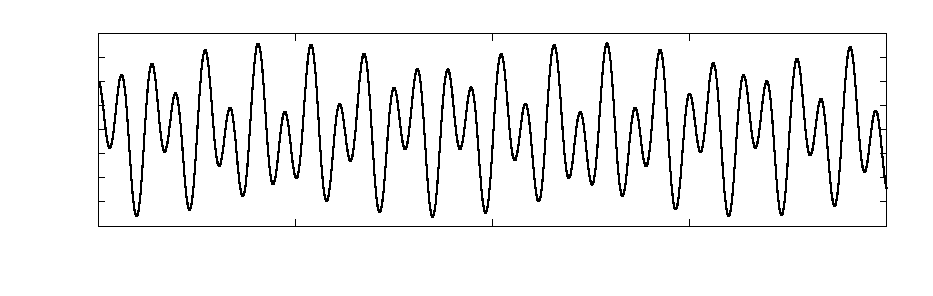
\includegraphics[width={432.00bp},height={126.00bp}]{images/omega05}}%
    \gplfronttext
  \end{picture}%
\endgroup

        \caption{Movement of the dipole with frequency of the external magnetic field being 0.5.}
        \label{fig:omega05}
    \end{subfigure}
    \begin{subfigure}{\textwidth}
        % GNUPLOT: LaTeX picture with Postscript
\begingroup
  \makeatletter
  \providecommand\color[2][]{%
    \GenericError{(gnuplot) \space\space\space\@spaces}{%
      Package color not loaded in conjunction with
      terminal option `colourtext'%
    }{See the gnuplot documentation for explanation.%
    }{Either use 'blacktext' in gnuplot or load the package
      color.sty in LaTeX.}%
    \renewcommand\color[2][]{}%
  }%
  \providecommand\includegraphics[2][]{%
    \GenericError{(gnuplot) \space\space\space\@spaces}{%
      Package graphicx or graphics not loaded%
    }{See the gnuplot documentation for explanation.%
    }{The gnuplot epslatex terminal needs graphicx.sty or graphics.sty.}%
    \renewcommand\includegraphics[2][]{}%
  }%
  \providecommand\rotatebox[2]{#2}%
  \@ifundefined{ifGPcolor}{%
    \newif\ifGPcolor
    \GPcolortrue
  }{}%
  \@ifundefined{ifGPblacktext}{%
    \newif\ifGPblacktext
    \GPblacktexttrue
  }{}%
  % define a \g@addto@macro without @ in the name:
  \let\gplgaddtomacro\g@addto@macro
  % define empty templates for all commands taking text:
  \gdef\gplbacktext{}%
  \gdef\gplfronttext{}%
  \makeatother
  \ifGPblacktext
    % no textcolor at all
    \def\colorrgb#1{}%
    \def\colorgray#1{}%
  \else
    % gray or color?
    \ifGPcolor
      \def\colorrgb#1{\color[rgb]{#1}}%
      \def\colorgray#1{\color[gray]{#1}}%
      \expandafter\def\csname LTw\endcsname{\color{white}}%
      \expandafter\def\csname LTb\endcsname{\color{black}}%
      \expandafter\def\csname LTa\endcsname{\color{black}}%
      \expandafter\def\csname LT0\endcsname{\color[rgb]{1,0,0}}%
      \expandafter\def\csname LT1\endcsname{\color[rgb]{0,1,0}}%
      \expandafter\def\csname LT2\endcsname{\color[rgb]{0,0,1}}%
      \expandafter\def\csname LT3\endcsname{\color[rgb]{1,0,1}}%
      \expandafter\def\csname LT4\endcsname{\color[rgb]{0,1,1}}%
      \expandafter\def\csname LT5\endcsname{\color[rgb]{1,1,0}}%
      \expandafter\def\csname LT6\endcsname{\color[rgb]{0,0,0}}%
      \expandafter\def\csname LT7\endcsname{\color[rgb]{1,0.3,0}}%
      \expandafter\def\csname LT8\endcsname{\color[rgb]{0.5,0.5,0.5}}%
    \else
      % gray
      \def\colorrgb#1{\color{black}}%
      \def\colorgray#1{\color[gray]{#1}}%
      \expandafter\def\csname LTw\endcsname{\color{white}}%
      \expandafter\def\csname LTb\endcsname{\color{black}}%
      \expandafter\def\csname LTa\endcsname{\color{black}}%
      \expandafter\def\csname LT0\endcsname{\color{black}}%
      \expandafter\def\csname LT1\endcsname{\color{black}}%
      \expandafter\def\csname LT2\endcsname{\color{black}}%
      \expandafter\def\csname LT3\endcsname{\color{black}}%
      \expandafter\def\csname LT4\endcsname{\color{black}}%
      \expandafter\def\csname LT5\endcsname{\color{black}}%
      \expandafter\def\csname LT6\endcsname{\color{black}}%
      \expandafter\def\csname LT7\endcsname{\color{black}}%
      \expandafter\def\csname LT8\endcsname{\color{black}}%
    \fi
  \fi
    \setlength{\unitlength}{0.0500bp}%
    \ifx\gptboxheight\undefined%
      \newlength{\gptboxheight}%
      \newlength{\gptboxwidth}%
      \newsavebox{\gptboxtext}%
    \fi%
    \setlength{\fboxrule}{0.5pt}%
    \setlength{\fboxsep}{1pt}%
    \definecolor{tbcol}{rgb}{1,1,1}%
\begin{picture}(8640.00,2520.00)%
    \gplgaddtomacro\gplbacktext{%
      \csname LTb\endcsname%%
      \put(592,512){\makebox(0,0)[r]{\strut{}$-70$}}%
      \put(592,743){\makebox(0,0)[r]{\strut{}$-60$}}%
      \put(592,974){\makebox(0,0)[r]{\strut{}$-50$}}%
      \put(592,1205){\makebox(0,0)[r]{\strut{}$-40$}}%
      \put(592,1436){\makebox(0,0)[r]{\strut{}$-30$}}%
      \put(592,1666){\makebox(0,0)[r]{\strut{}$-20$}}%
      \put(592,1897){\makebox(0,0)[r]{\strut{}$-10$}}%
      \put(592,2128){\makebox(0,0)[r]{\strut{}$0$}}%
      \put(592,2359){\makebox(0,0)[r]{\strut{}$10$}}%
      \put(784,352){\makebox(0,0){\strut{}$0$}}%
      \put(2676,352){\makebox(0,0){\strut{}$50$}}%
      \put(4568,352){\makebox(0,0){\strut{}$100$}}%
      \put(6459,352){\makebox(0,0){\strut{}$150$}}%
      \put(8351,352){\makebox(0,0){\strut{}$200$}}%
    }%
    \gplgaddtomacro\gplfronttext{%
      \csname LTb\endcsname%%
      \put(152,1435){\rotatebox{-270}{\makebox(0,0){\strut{}$\theta (t)$}}}%
      \put(4519,112){\makebox(0,0){\strut{}Time}}%
    }%
    \gplbacktext
    \put(0,0){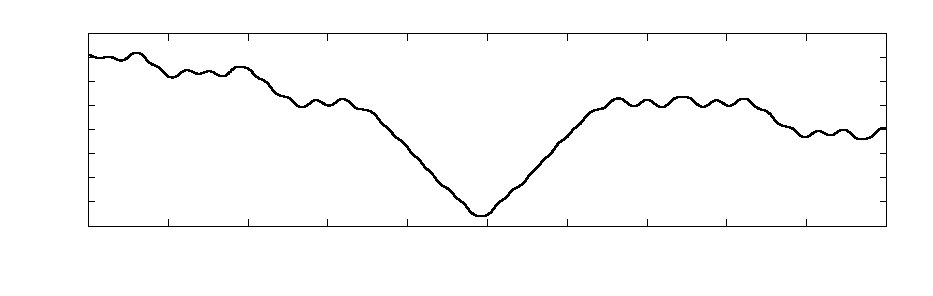
\includegraphics[width={432.00bp},height={126.00bp}]{images/omega075}}%
    \gplfronttext
  \end{picture}%
\endgroup

        \caption{Movement of the dipole with frequency of the external magnetic field being 0.75.}
        \label{fig:omega075}
    \end{subfigure}
    \begin{subfigure}{\textwidth}
        % GNUPLOT: LaTeX picture with Postscript
\begingroup
  \makeatletter
  \providecommand\color[2][]{%
    \GenericError{(gnuplot) \space\space\space\@spaces}{%
      Package color not loaded in conjunction with
      terminal option `colourtext'%
    }{See the gnuplot documentation for explanation.%
    }{Either use 'blacktext' in gnuplot or load the package
      color.sty in LaTeX.}%
    \renewcommand\color[2][]{}%
  }%
  \providecommand\includegraphics[2][]{%
    \GenericError{(gnuplot) \space\space\space\@spaces}{%
      Package graphicx or graphics not loaded%
    }{See the gnuplot documentation for explanation.%
    }{The gnuplot epslatex terminal needs graphicx.sty or graphics.sty.}%
    \renewcommand\includegraphics[2][]{}%
  }%
  \providecommand\rotatebox[2]{#2}%
  \@ifundefined{ifGPcolor}{%
    \newif\ifGPcolor
    \GPcolortrue
  }{}%
  \@ifundefined{ifGPblacktext}{%
    \newif\ifGPblacktext
    \GPblacktexttrue
  }{}%
  % define a \g@addto@macro without @ in the name:
  \let\gplgaddtomacro\g@addto@macro
  % define empty templates for all commands taking text:
  \gdef\gplbacktext{}%
  \gdef\gplfronttext{}%
  \makeatother
  \ifGPblacktext
    % no textcolor at all
    \def\colorrgb#1{}%
    \def\colorgray#1{}%
  \else
    % gray or color?
    \ifGPcolor
      \def\colorrgb#1{\color[rgb]{#1}}%
      \def\colorgray#1{\color[gray]{#1}}%
      \expandafter\def\csname LTw\endcsname{\color{white}}%
      \expandafter\def\csname LTb\endcsname{\color{black}}%
      \expandafter\def\csname LTa\endcsname{\color{black}}%
      \expandafter\def\csname LT0\endcsname{\color[rgb]{1,0,0}}%
      \expandafter\def\csname LT1\endcsname{\color[rgb]{0,1,0}}%
      \expandafter\def\csname LT2\endcsname{\color[rgb]{0,0,1}}%
      \expandafter\def\csname LT3\endcsname{\color[rgb]{1,0,1}}%
      \expandafter\def\csname LT4\endcsname{\color[rgb]{0,1,1}}%
      \expandafter\def\csname LT5\endcsname{\color[rgb]{1,1,0}}%
      \expandafter\def\csname LT6\endcsname{\color[rgb]{0,0,0}}%
      \expandafter\def\csname LT7\endcsname{\color[rgb]{1,0.3,0}}%
      \expandafter\def\csname LT8\endcsname{\color[rgb]{0.5,0.5,0.5}}%
    \else
      % gray
      \def\colorrgb#1{\color{black}}%
      \def\colorgray#1{\color[gray]{#1}}%
      \expandafter\def\csname LTw\endcsname{\color{white}}%
      \expandafter\def\csname LTb\endcsname{\color{black}}%
      \expandafter\def\csname LTa\endcsname{\color{black}}%
      \expandafter\def\csname LT0\endcsname{\color{black}}%
      \expandafter\def\csname LT1\endcsname{\color{black}}%
      \expandafter\def\csname LT2\endcsname{\color{black}}%
      \expandafter\def\csname LT3\endcsname{\color{black}}%
      \expandafter\def\csname LT4\endcsname{\color{black}}%
      \expandafter\def\csname LT5\endcsname{\color{black}}%
      \expandafter\def\csname LT6\endcsname{\color{black}}%
      \expandafter\def\csname LT7\endcsname{\color{black}}%
      \expandafter\def\csname LT8\endcsname{\color{black}}%
    \fi
  \fi
    \setlength{\unitlength}{0.0500bp}%
    \ifx\gptboxheight\undefined%
      \newlength{\gptboxheight}%
      \newlength{\gptboxwidth}%
      \newsavebox{\gptboxtext}%
    \fi%
    \setlength{\fboxrule}{0.5pt}%
    \setlength{\fboxsep}{1pt}%
    \definecolor{tbcol}{rgb}{1,1,1}%
\begin{picture}(8640.00,2520.00)%
    \gplgaddtomacro\gplbacktext{%
      \csname LTb\endcsname%%
      \put(688,512){\makebox(0,0)[r]{\strut{}$-1.5$}}%
      \put(688,820){\makebox(0,0)[r]{\strut{}$-1$}}%
      \put(688,1128){\makebox(0,0)[r]{\strut{}$-0.5$}}%
      \put(688,1436){\makebox(0,0)[r]{\strut{}$0$}}%
      \put(688,1743){\makebox(0,0)[r]{\strut{}$0.5$}}%
      \put(688,2051){\makebox(0,0)[r]{\strut{}$1$}}%
      \put(688,2359){\makebox(0,0)[r]{\strut{}$1.5$}}%
      \put(784,352){\makebox(0,0){\strut{}$0$}}%
      \put(2676,352){\makebox(0,0){\strut{}$50$}}%
      \put(4568,352){\makebox(0,0){\strut{}$100$}}%
      \put(6459,352){\makebox(0,0){\strut{}$150$}}%
      \put(8351,352){\makebox(0,0){\strut{}$200$}}%
    }%
    \gplgaddtomacro\gplfronttext{%
      \csname LTb\endcsname%%
      \put(152,1435){\rotatebox{-270}{\makebox(0,0){\strut{}$\theta (t)$}}}%
      % \put(4567,112){\makebox(0,0){\strut{}Time}}%
    }%
    \gplbacktext
    \put(0,0){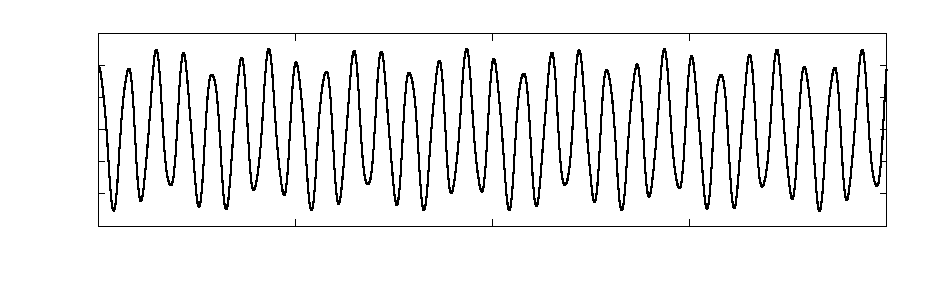
\includegraphics[width={432.00bp},height={126.00bp}]{images/omega20}}%
    \gplfronttext
  \end{picture}%
\endgroup

        \caption{Movement of the dipole with frequency of the external magnetic field being 2.0.}
        \label{fig:omega20}
    \end{subfigure}
    \caption{Movement of the dipole for different frequencies of the magnetic field. Using $\varepsilon = 0.5$}
\end{figure*}

\listoffigures

\bibliographystyle{unsrt}
\bibliography{bibliography/bibfile}

\end{document}